\section{Hermite Algorithm for Periodicity Detection (\HAPD)}\label{sec:hapd_algorithm}

\begin{figure}[htbp]
\begin{minipage}{\textwidth}
\centering
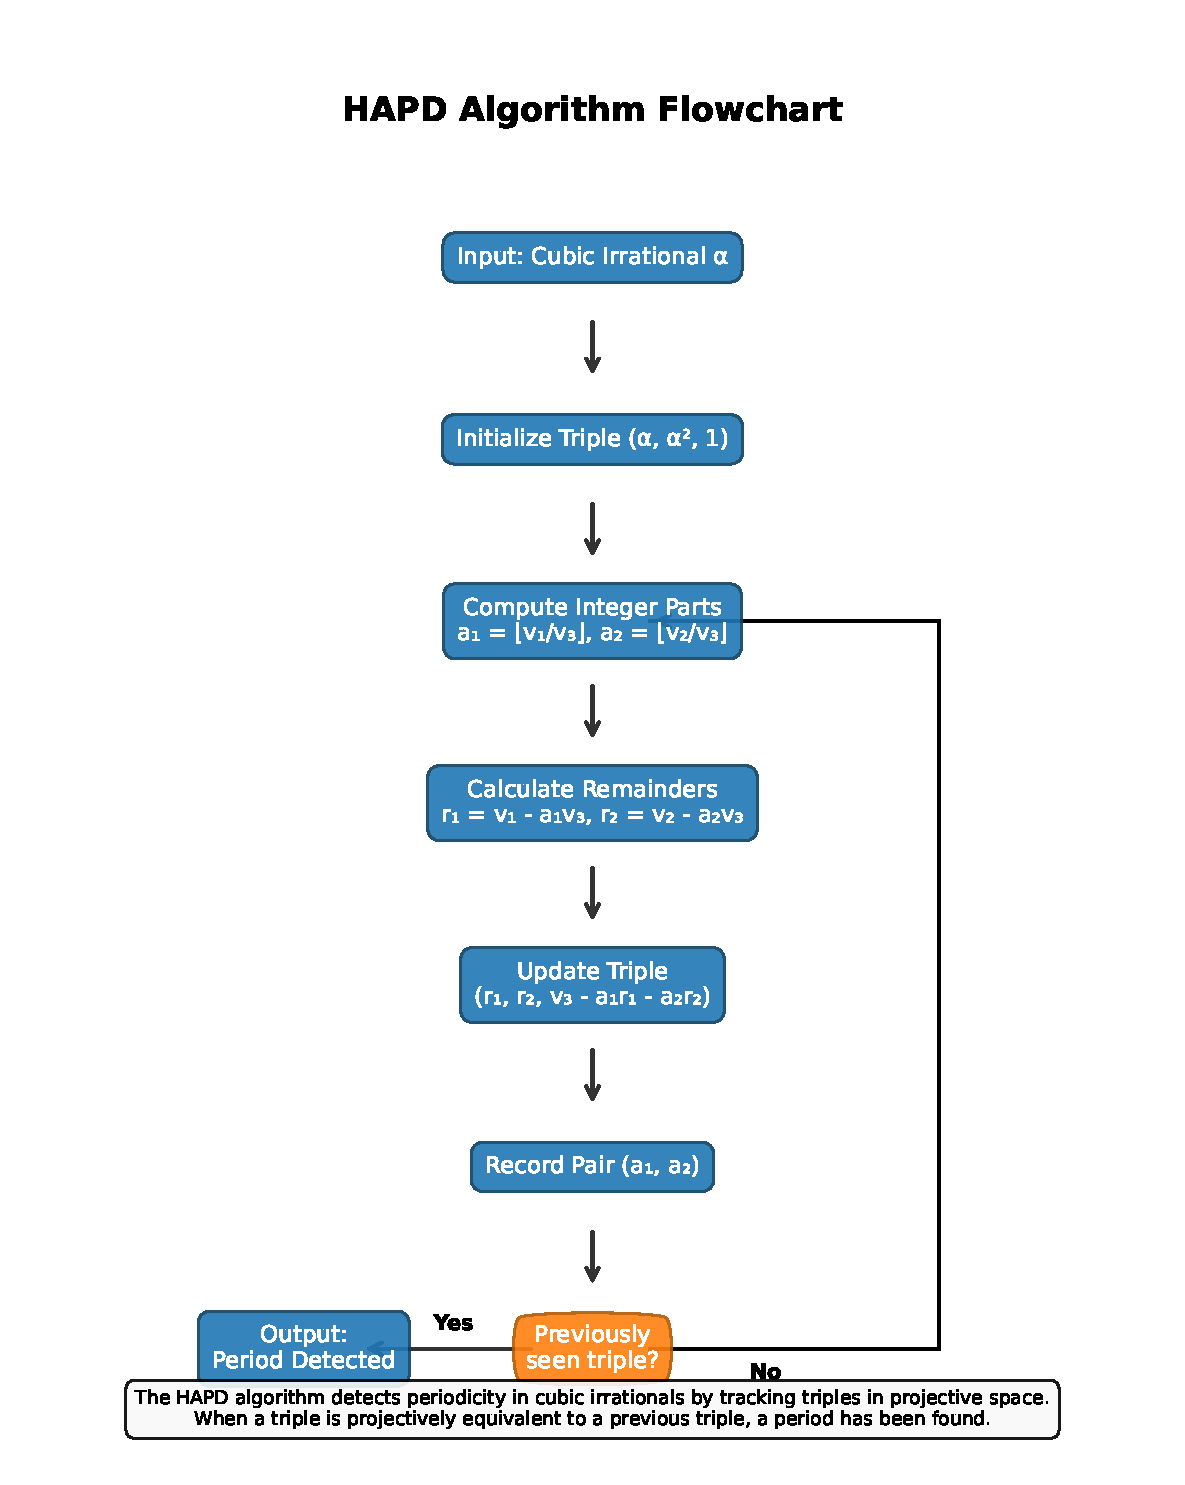
\includegraphics[width=\textwidth]{figures/output/hapd_algorithm_flowchart.pdf}
\caption{HAPD algorithm flowchart.}
\label{fig:hapd_flowchart}
\end{minipage}
\end{figure}

\begin{figure}[htbp]
\begin{minipage}{\textwidth}
\centering
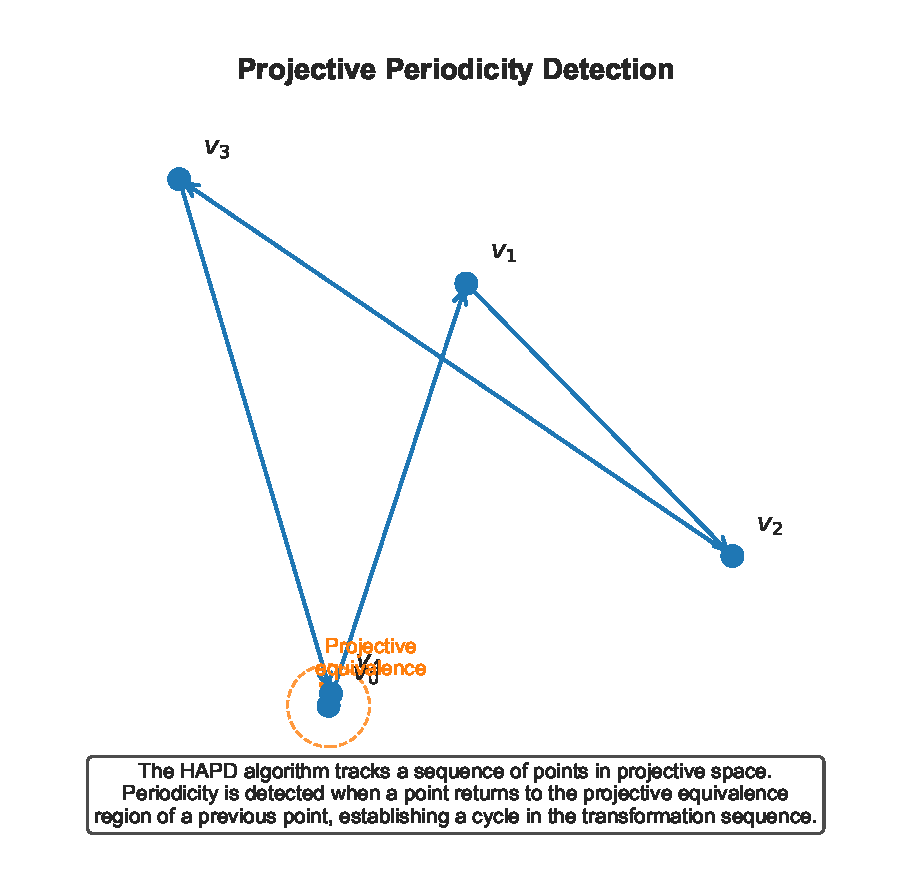
\includegraphics[width=\textwidth]{figures/output/projective_periodicity_visualization.pdf}
\caption{Periodicity detection in projective space: $v_4$ returns to the equivalence region of $v_0$.}
\label{fig:projective_visualization}
\end{minipage}
\end{figure}

\begin{figure}[htbp]
\begin{minipage}{\textwidth}
\centering
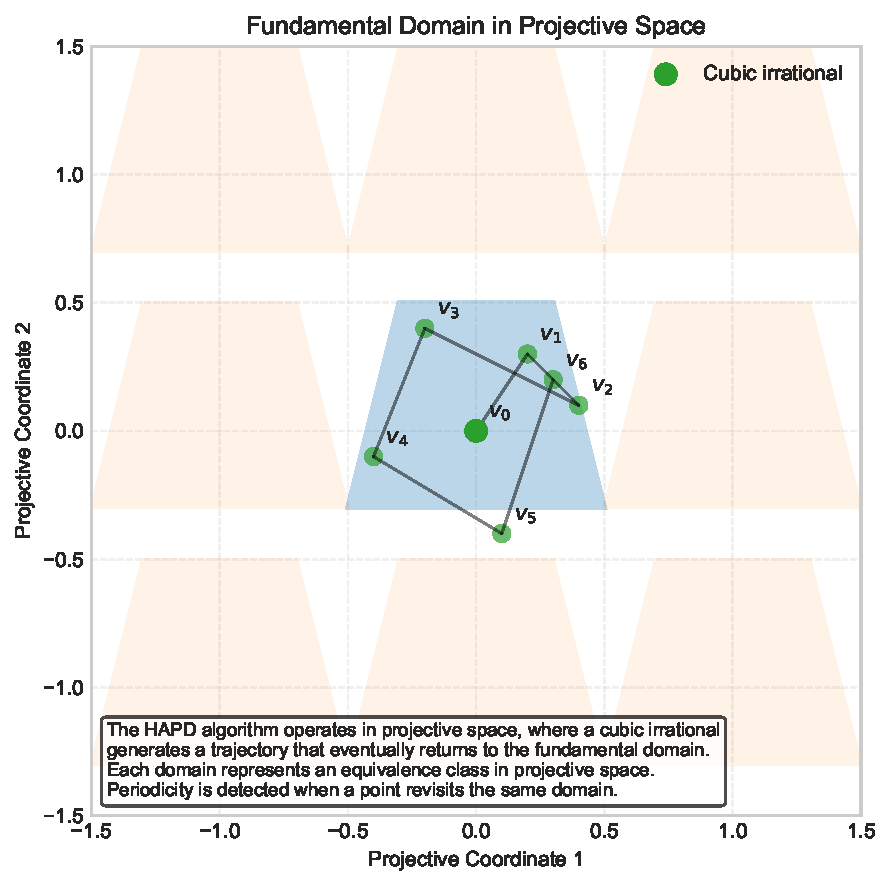
\includegraphics[width=\textwidth]{figures/projective_space_regions.pdf}
\caption{Projective trajectory for $\sqrt{^3}{2}$: $v_{11}$ returns to $v_4$ class, establishing period 7.}
\label{fig:projective_trajectory}
\end{minipage}
\end{figure}

\subsection{Algorithm Definition}

\begin{algorithm_def}[\HAPD{} Algorithm]\label{alg:hapd}
For any real number $\alpha$:
\begin{enumerate}
    \item Initialize with $(v_1, v_2, v_3) = (\alpha, \alpha^2, 1)$
    \item Iterate:
    \begin{enumerate}
        \item Compute integer parts $a_1 = \floor{v_1/v_3}$, $a_2 = \floor{v_2/v_3}$
        \item Calculate remainders $r_1 = v_1 - a_1v_3$, $r_2 = v_2 - a_2v_3$
        \item Update $(v_1, v_2, v_3) \leftarrow (r_1, r_2, v_3 - a_1r_1 - a_2r_2)$
        \item Record $(a_1, a_2)$
    \end{enumerate}
    \item Encode each pair $(a_1, a_2)$ using injective function $E$
\end{enumerate}
\end{algorithm_def}

\begin{definition}[Encoding Function]\label{def:encoding}
$E : \Z^2 \to \N$ defined as $E(a, b) = 2^{|a|} \cdot 3^{|b|} \cdot 5^{(\operatorname{sgn}(a)+1)} \cdot 7^{(\operatorname{sgn}(b)+1)}$.
\end{definition}

\begin{proposition}[Computational Complexity]\label{prop:complexity}
For a cubic irrational with minimal polynomial coefficients bounded by $M$, HAPD requires $O(M^3)$ iterations to detect periodicity, each iteration performing $O(1)$ arithmetic operations.
\end{proposition}

\begin{lemma}[Injectivity of Encoding]\label{lem:encoding_injective}
The encoding function $E$ is injective.
\end{lemma}

\begin{proof}
$E$ uses unique factorization. Components affect different primes: $|a| \to 2^k$, $|b| \to 3^k$, $\operatorname{sgn}(a) \to 5^k$, $\operatorname{sgn}(b) \to 7^k$.
\end{proof}

\subsection{Projective Geometry Interpretation}

\begin{definition}[Projective Space $\mathbb{P}^2(\mathbb{R})$ \cite{KarpenkovBook}]
$\mathbb{P}^2(\mathbb{R})$ is the set of equivalence classes of non-zero triples $(x : y : z) \in \mathbb{R}^3 \setminus \{(0,0,0)\}$ under $(x : y : z) \sim (\lambda x : \lambda y : \lambda z)$ for $\lambda \neq 0$.
\end{definition}

\begin{proposition}[Projective Invariance]\label{prop:projective_invariance}
HAPD transformation preserves projective structure.
\end{proposition}

\begin{proof}
Let $\lambda \neq 0$. Consider $(v_1, v_2, v_3)$ and $(\lambda v_1, \lambda v_2, \lambda v_3)$. Integer parts $\floor{\lambda v_1/\lambda v_3} = \floor{v_1/v_3}$ and $\floor{\lambda v_2/\lambda v_3} = \floor{v_2/v_3}$ are preserved. Remainders and new $v_3$ scale by $\lambda$, preserving projective equivalence.
\end{proof}

\begin{definition}[Dirichlet Group \cite{Karpenkov2022}]
A Dirichlet group $\Gamma$ for cubic field $K$ is a discrete subgroup of $\GL(3,\mathbb{R})$ preserving the field structure.
\end{definition}

\begin{theorem}[Finiteness of Fundamental Domain \cite{Karpenkov2022}]\label{thm:finite_domain}
For cubic field $K$, the Dirichlet group $\Gamma_K$ has a fundamental domain of finite volume in $\mathbb{P}^2(\mathbb{R})$.
\end{theorem}

\subsection{Main Periodicity Theorem}

\begin{theorem}[Cubic Irrationals Yield Periodic Sequences]\label{thm:cubic_periodic}
If $\alpha$ is a cubic irrational, the HAPD sequence is eventually periodic.
\end{theorem}

\begin{proof}
Let $\alpha$ be a cubic irrational. Start with $(\alpha, \alpha^2, 1)$.
\begin{enumerate}
    \item HAPD transformation preserves the cubic field structure $\Q(\alpha)$.
    \item By Prop. \ref{prop:projective_invariance}, the transformation is linear fractional in projective space.
    \item By Thm. \ref{thm:finite_domain}, the Dirichlet group $\Gamma_{\Q(\alpha)}$ has a finite volume fundamental domain $F$.
    \item By pigeonhole principle \cite{Schmidt1980}, the sequence must revisit an equivalence class: $(v^{(m)}) \sim (v^{(n)})$ for $m < n$.
\end{enumerate}
Revisiting an equivalence class causes subsequent transformations to repeat, yielding periodicity.
\end{proof}

\begin{theorem}[Only Cubic Irrationals Yield Periodic Sequences]\label{thm:only_cubic_periodic}
If the HAPD sequence for $\alpha$ is eventually periodic, then $\alpha$ is a cubic irrational.
\end{theorem}

\begin{proof}
Consider cases:
\textbf{Case 1: $\alpha$ is rational.} HAPD terminates (division by zero or undefined values) due to zero fractional parts.
\textbf{Case 2: $\alpha$ is quadratic irrational.} Minimal polynomial $x^2+px+q=0$ implies $\alpha^2 = -p\alpha - q$. Triple $(\alpha, \alpha^2, 1)$ lies in subspace $v_2 = -pv_1 - qv_3$. HAPD preserves this, but the group action lacks a finite fundamental domain in the relevant projective subspace \cite{Khinchin1964}.
\end{proof}
